\documentclass{article}
\usepackage{graphicx} % Required for inserting images

\title{Checkpoint One Report}
\author{ Team 2}
\date{January 2024}

\begin{document}

\maketitle

\section{Introduction}
The purpose of this document is to express our findings and understanding of what the first milestone asks for. The milestone is split into two parts; task one instructs the team to read through a paper and summarize our findings. The second task is to perform Exploratory Data Analysis(EDA) on the data set used.

\section{Task One}
The paper was written by researches at Stanford University and focuses on predicting drug response, targets, and side effects. The researchers created Drug Orchestra. Drug Orchestra uses a deep learning multi task learning(MTL) model to assist in pharmacogenomics. Pharmacogenomics is the study of how a person’s genes affect their response to drugs. The importance of this field stems from safety; the creation of a medical drug that is safe for all to use and has minimal side effects is the end goal. The key idea of MTL is to solve multiple prediction tasks at the same time while automatically exploiting similarities and differences across tasks. This predicts drug response, targets, and side effects. It address the predicting of drug response, drug targets, and drug side effects in pharmacogenomics. Their proposed  idea is Drug Orchestra which is a multi-task learning method that predicts drug respond, targets and side effects. The data sets used to create Drug Orchestra was sourced from many locations and serve different purposes. They come from Drug Bank, PDX, CCLE, SIDER, OFFSIDES, GDSC, STITCH, and Repurposing Hub. For instance, drug targets used the Repurposing Hub, PDX, and Sider with much overlap. In the end, the goal for using these data sets is to train Drug Orchestra to train the model in predicting the side effects given a certain amount of genes. To do this, a random forest was implemented. The architecture included three predictions: drug target, drug response, and drug side effects. Each prediction will take two inputs, drug feature being static in all three and gene feature, cell line feature, and disease feature being variable based on the respective predictions. There are multiple decision trees with dynamic weight adjustment that will lead to a certain output which is the prediction. The conclusion of the experiment resulted in positive results. Drug Orchestra was able to successfully predict the target, response, and side effect given the genes that were subjected to the drug.

\section{Task Two}
The second task was to perform EDA. There were many files from each data set listed in the Standford report. The two versions of the data drive was a summarized version and a much longer raw version. The raw version contained columns of float values that led to different categories to aid in training the model. The raw versions were incredibly large files, figure 1, as well. Due to memory issues from how large the files were, EDA had to be done on the broken up pieces of the raw data and the summarized version. 
\begin{figure}
    \centering
    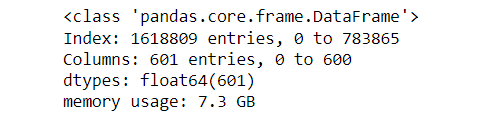
\includegraphics[width=0.5\linewidth]{1.png}
    \caption{Info command for Sider, CCLE, Drug Bank, and GDSC}
    \label{fig:enter-label}
\end{figure}
The summarized version was split up into separate categories based on the intention of the researchers. Figure two shows the relationship between the variables LN18 and 769P. There appears to be no correlation. There appears to be no discernible pattern or significant link between the two variables when the dots are dispersed randomly.
\begin{figure}
    \centering
    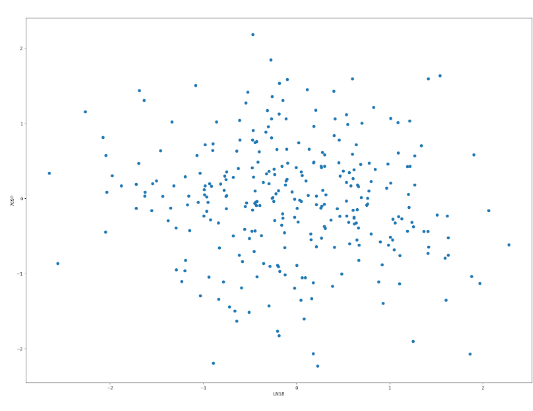
\includegraphics[width=0.5\linewidth]{2.png}
    \caption{LN18 and 769P relationship}
    \label{fig:enter-label}
\end{figure}
Box plots were further used to get a better understanding of how disperse the data is. This dispersion will prove useful to ensure the model can withstand all types of data.
\begin{figure}
    \centering
    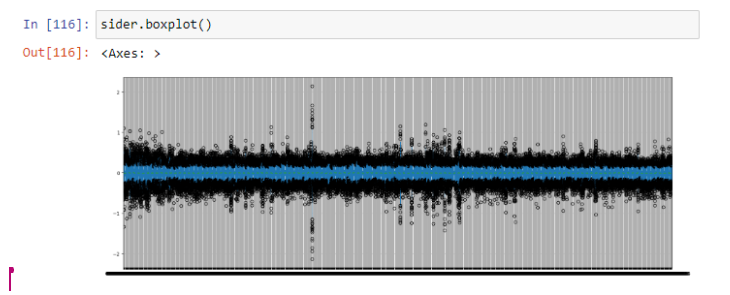
\includegraphics[width=0.5\linewidth]{3.png}
    \caption{Box Plot for Sider}
    \label{fig:enter-label}
\end{figure}
\section{Conclusion}
The purpose of this milestone was to understand and summarize a research paper and conduct EDA on the data used to to create that paper. EDA showed that the distribution of data the researchers used to create Drug Orchestra would better train it using decision trees. Furthermore, it would handle and better predict response, target, and side effects of drugs given a type of gene set. The milestone proved useful in practicing EDA on larger, more complex, real world data sets.
\end{document}
